\documentclass[aspectratio=169,11pt]{beamer}

% Shared style (ib-tutorials.sty at the repo root).
\makeatletter\def\input@path{{./}{../}}\makeatother
\usepackage{ib-tutorials}

\usepackage[utf8]{inputenc}
\usepackage{amsmath,amssymb}
\usepackage{booktabs}
\usepackage{array}
\newcolumntype{L}[1]{>{\raggedright\arraybackslash}p{#1}}
\usepackage{graphicx}
\graphicspath{{../pictures/2-ib2d/}{pictures/2-ib2d/}}
\usepackage{xcolor}
\usepackage{listings}
\usepackage{tikz}
\usetikzlibrary{arrows.meta,positioning,shapes.geometric,fit,calc}
\usepackage{hyperref}

\newcommand{\sourcecredit}[1]{\vfill\hfill{\tiny\textcolor{DarkGray}{#1}}}
\newcommand{\gui}[1]{\textsf{\textbf{#1}}}

\lstset{
  basicstyle=\ttfamily\scriptsize\color{BlackGray},
  keywordstyle=\color{NavyBlue}\bfseries,
  commentstyle=\color{DarkGray}\itshape,
  stringstyle=\color{OliveGreen},
  showstringspaces=false,
  columns=fullflexible,
  keepspaces=true,
  breaklines=true,
  frame=single,
  framerule=0.4pt,
  rulecolor=\color{LightGray},
  backgroundcolor=\color{LightGray!30},
  xleftmargin=0.25em,
  xrightmargin=0.25em
}
\lstdefinestyle{shell}{morecomment=[l]{\#}}
\lstdefinestyle{input}{morecomment=[l]{\%}}
\lstdefinestyle{plain}{}
\lstdefinestyle{py}{language=Python}
\lstdefinestyle{tiny}{basicstyle=\ttfamily\tiny\color{BlackGray}}
\lstdefinestyle{pytiny}{language=Python,basicstyle=\ttfamily\tiny\color{BlackGray}}

\title[IB2d: meshes from images]{Meshes from images: MeshmerizeMe}
\subtitle{From a photograph to Lagrangian points at $\Delta s = \Delta x/2$: ContourizeMe's contours, SVG paths and B\'ezier curves, MeshmerizeMe's equal-distance points; checked against the files IB2d ships, reproduced with a small sampler, and run as a starfish in a channel}
\author[Miller]{Laura A. Miller}
\institute[UArizona]{Department of Mathematics, University of Arizona}
\date{Using IB Software \textbullet\ Part II \textbullet\ Chapter 4f}

\begin{document}

% ---------------------------------------------------------------- title
\begin{frame}[plain]
\maketutorialtitlepanel{%
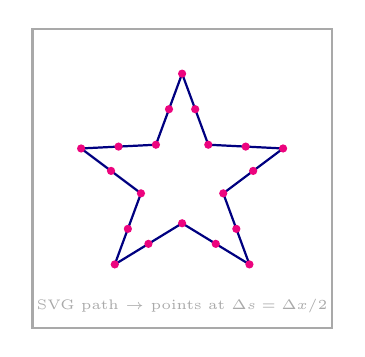
\begin{tikzpicture}[scale=0.95]
  \draw[DarkGray,thick] (0,0) rectangle (4,4);
  \draw[NavyBlue,thick] (2,3.4) -- (2.35,2.45) -- (3.35,2.4) -- (2.55,1.8) -- (2.9,0.85) -- (2,1.4) -- (1.1,0.85) -- (1.45,1.8) -- (0.65,2.4) -- (1.65,2.45) -- cycle;
  \foreach \p in {(2,3.4),(2.175,2.925),(2.35,2.45),(2.85,2.425),(3.35,2.4),(2.95,2.1),(2.55,1.8),(2.725,1.325),(2.9,0.85),(2.45,1.125),(2,1.4),(1.55,1.125),(1.1,0.85),(1.275,1.325),(1.45,1.8),(1.05,2.1),(0.65,2.4),(1.15,2.425),(1.65,2.45),(1.825,2.925)} {\fill[RubineRed] \p circle (0.055);}
  \node[font=\tiny,DarkGray] at (2,0.3) {SVG path $\to$ points at $\Delta s = \Delta x/2$};
\end{tikzpicture}}
\end{frame}

% ---------------------------------------------------------------- goals, sources
\begin{frame}{What you will be able to do after this chapter}
\label{fr:goals}
\footnotesize
\begin{itemize}
  \item Describe the MeshmerizeMe workflow: an image, contours found by ContourizeMe, an SVG file cleaned or drawn in a vector editor, and MeshmerizeMe's \code{.vertex} file at the spacing $\Delta s = \Delta x/2$ the immersed boundary method wants.
  \item Read SVG path data (the commands, relative coordinates, the smooth curves, the arcs), evaluate B\'ezier curves and their arc length, and map SVG coordinates to the simulation box.
  \item Explain how MeshmerizeMe places the points (equal Euclidean distances, found by gradient descent) and what its errors are; check a \code{.vertex} file's spacing yourself.
  \item Turn a \code{.vertex} file into an IB2d example: targets, walls, a driven flow; and know what the IB2d starfish example does with its points, and what it does not.
\end{itemize}
\begin{punchbox}
\small MeshmerizeMe itself is not installed on this tutorial's laptop. This chapter describes it from its paper, the 2021 lecture and Senter's design notes, measures the MeshmerizeMe output that ships with IB2d, and does the same job (points at equal Euclidean distances, found by a walk and bisection instead of MeshmerizeMe's gradient descent) with a 400-line script (\code{examples/IB2d/Mesh\_From\_SVG/svg\_to\_vertex.py}, about 320 lines of code) whose output then runs in Python IB2d (October 2026).
\end{punchbox}
\end{frame}

\begin{frame}{Where this chapter comes from}
\label{fr:sources}
\footnotesize
\begin{itemize}
  \item \al{``MeshMerizeMe'' (June 2021, 7 slides):} the project's GitHub page (\url{https://github.com/dmsenter89/MeshmerizeMe}, ``Software to create 2D geometry for IBAMR and IB2D''), installation, ContourizeMe's usage, MeshmerizeMe's usage, each pointing to the project's documentation pages (slide 4: ``See the project wiki''); and the paper.
  \item \al{D.\,M. Senter, D.\,R. Douglas, W.\,C. Strickland, S.\,G. Thomas, A.\,M. Talkington, L.\,A. Miller, N.\,A. Battista, ``A semi-automated finite difference mesh creation method for use with immersed boundary software IB2d and IBAMR'', Bioinspir.\ Biomim.\ 16 (2021) 016008:} the workflow, ContourizeMe's image processing, MeshmerizeMe's discretisation and its errors, and three examples.
  \item \al{M. Senter, ``Creating a Curvilinear Mesh from B\'ezier Curves'' (design notes for an early C++ version, UNC, about 2017, 20 pages):} B\'ezier curves, de Casteljau, arc length, SVG path data and primitives, the map from SVG space to the experiment.
  \item \al{IB2d's \code{matIB2d/Examples/Example\_Meshmerize\_Me}:} the dragonfly wing, insect wing veins, leaf and starfish examples, their SVG files and MATLAB scripts, the MeshmerizeMe output for the starfish and the wing, and an unfinished \code{MeshingTutorial.md}.
\end{itemize}
What is new here: the starfish files measured; the design notes' arc-length rule tested; a small sampler written, tested on IB2d's SVGs, and used to build the starfish example in Python, which ran; four things about the shipped starfish example found on the way.
\end{frame}

% ---------------------------------------------------------------- why
\begin{frame}{Why a mesher for the immersed boundary method}
\label{fr:why}
\small
\begin{itemize}
  \item Many IB studies are done in 2D with shapes that have formulas (plates, strings, tubes, ellipses, hemi-ellipses, circles); anything else has to be built point by point or from piecewise functions, which is ``non-trivial''. The paper quotes a Pixar scientist: ``I hate meshes. I cannot believe how hard this is.''
  \item Mesh generators (MeshLab, Gmsh, TetGen) make \al{finite element} meshes (chapter 18). The classic IB method needs a \al{finite difference} curve: points along the boundary about $\Delta s = \Delta x/2$ apart, in order, in the simulation's coordinates.
  \item Biology often comes with images: a photograph, a micrograph, a scan. The geometry is in the picture; the work is getting it out.
\end{itemize}
\begin{punchbox}
\small The paper's examples: hemolymph through dragonfly wing veins (IB2d, a sweep of $Re$ over $[0.1, 100]$, shown at 0.6, 6 and 60), lymph through a branching lymphatic capillary of a mouse embryo (IBAMR), oscillatory flow past one, three and five starfish (IB2d, $Re = 800$); and, before the paper, blood flow over the trabeculae of zebrafish embryonic hearts.
\end{punchbox}
\sourcecredit{Senter et al.\ (2021), sections 1, 3 and 4.}
\end{frame}

\begin{frame}{The workflow}
\label{fr:workflow}
\centering
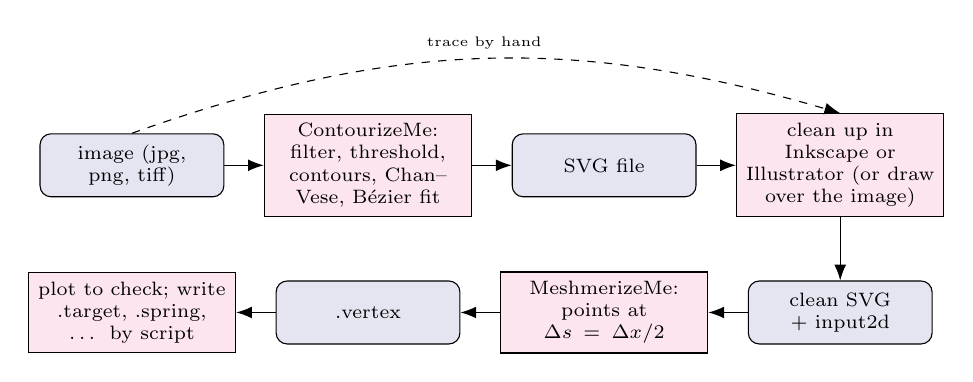
\begin{tikzpicture}[node distance=4mm and 5mm, every node/.style={font=\scriptsize, align=center}]
  \tikzset{file/.style={draw,rounded corners=4pt,fill=NavyBlue!10,minimum height=8mm,text width=2.1cm}, act/.style={draw,fill=RubineRed!10,minimum height=8mm,text width=2.4cm}}
  \node[file] (img) {image (jpg, png, tiff)};
  \node[act,right=of img] (ci) {ContourizeMe: filter, threshold, contours, Chan--Vese, B\'ezier fit};
  \node[file,right=of ci] (svg) {SVG file};
  \node[act,right=of svg] (clean) {clean up in Inkscape or Illustrator (or draw over the image)};
  \node[file,below=8mm of clean] (svg2) {clean SVG + \code{input2d}};
  \node[act,left=of svg2] (mm) {MeshmerizeMe: points at $\Delta s = \Delta x/2$};
  \node[file,left=of mm] (vtx) {\code{.vertex}};
  \node[act,left=of vtx] (phys) {plot to check; write \code{.target}, \code{.spring}, \ldots{} by script};
  \foreach \u/\v in {img/ci,ci/svg,svg/clean,clean/svg2,svg2/mm,mm/vtx,vtx/phys} {\draw[-{Latex[length=2mm]}] (\u) -- (\v);}
  \draw[-{Latex[length=2mm]},dashed] (img.north) to[bend left=18] node[above,font=\tiny] {trace by hand} (clean.north);
\end{tikzpicture}

\vspace{3mm}
\small Two entry points: automatic edge detection with ContourizeMe, or an SVG drawn by hand over the image (when there is no image, the image is poor, or the shape is hypothetical). Either way the SVG is the interface: any vector editor can fix it. MeshmerizeMe only makes the points; which points are springs, beams or targets is written by a script afterwards (a few of these relations are classes in the MeshmerizeMe library).
\sourcecredit{After figure 1 of Senter et al.\ (2021) (blue: files; red: actions), redrawn.}
\end{frame}

% ---------------------------------------------------------------- ContourizeMe
\begin{frame}[fragile]{ContourizeMe: from pixels to curves}
\label{fr:contourize}
\begin{columns}[T]
\column{0.5\textwidth}
\scriptsize
A Tkinter GUI started from the command line on an image (jpg, png, tiff):
\begin{lstlisting}[style=shell]
ContourizeMe image.jpg
# usage: ContourizeMe [-h] image
\end{lstlisting}
\begin{itemize}
  \item choose a parameterisation of the pixels: grayscale, RGB or HSV; sliders set the threshold bounds (one for grayscale, three for RGB and HSV) and update the detected edges live (green);
  \item optional contrast and saturation changes (temporary) and \al{noise reduction}: average, Gaussian, median, or the recommended \al{bilateral} filter (it weights pixels by intensity difference as well as distance, to keep edges);
  \item the thresholded binary image goes to OpenCV's topological contour algorithm (integer pixel boundaries), refined to sub-pixel with the \al{Chan--Vese} algorithm at a chosen smoothness; B\'ezier curves through evenly spaced points of the refined boundary are written to an SVG file.
\end{itemize}
\column{0.48\textwidth}
\scriptsize
\al{What makes a good image:} a strong contrast between the object and the background, and little noise; otherwise the sliders and filters, then deleting stray edges by hand.

\al{What comes out:} one tiny path per cubic piece. The starfish of the IB2d example: 3996 \code{<path>} elements, each \code{M x,y C \ldots}, with \code{stroke-width} and \code{fill="none"}; the coordinates are the image's pixels, but the drawing's \code{viewBox} is the contours' bounding box enlarged by about 20\,\% (a 10\,\% margin on each side), not the image's frame: the starfish's starts at $(102.08, 20.94)$, the dragonfly wing's at $x = -46.75$.

\al{The IB2d dragonfly example's folder} keeps the intermediate pictures: \code{Images/cropped\_wing\_v3.png}, the Chan--Vese result \code{chanvese\_contour.png}, and the SVG.
\end{columns}
\sourcecredit{The 2021 lecture, slide 6; Senter et al.\ (2021), section 2.1 and figure 2.}
\end{frame}

\begin{frame}{Cleaning the SVG: the starfish before and after}
\label{fr:clean}
\centering
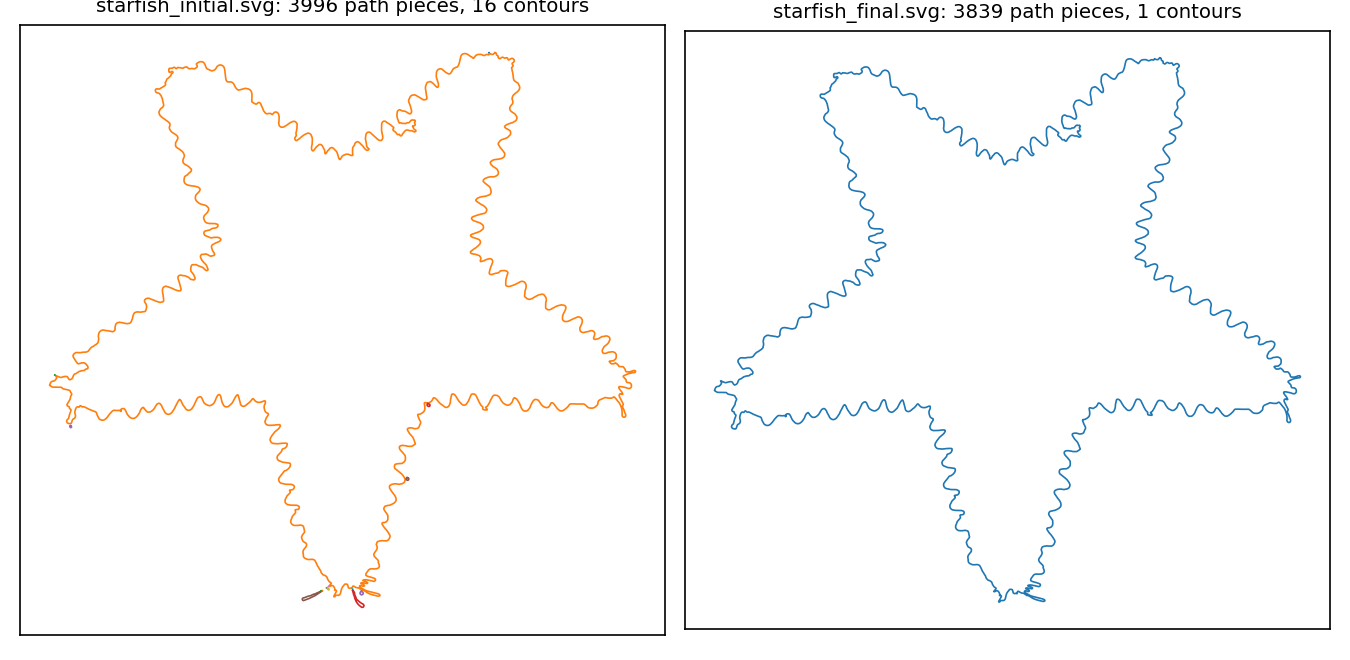
\includegraphics[width=0.62\textwidth]{ch4f-svg-cleaning.png}

\scriptsize
\begin{columns}[T]
\column{0.5\textwidth}
Left: ContourizeMe's output (\code{starfish\_initial.svg}): 3996 pieces that join into 16 contours, the starfish (5950 SVG units long) and 15 small loops of noise (73 units and less). Right: the cleaned file (\code{starfish\_final.svg}): 3839 pieces, one closed contour. (The cleaned version saved by Inkscape, \code{starfish\_cleaned.svg}, holds the same curve.)
\column{0.48\textwidth}
The paper's advice: delete curves that come from background noise; collapse groups and simplify contiguous paths (a ``save'' option of some editors, or SVGO / SVGOMG); give each object one contiguous path. MeshmerizeMe merges all paths of a file into one poly-B\'ezier curve: two separate objects in one file give a long jump between them and a large error.
\end{columns}
\sourcecredit{\code{tools/ch4f\_figures.py}; the SVG files of \code{Example\_Meshmerize\_Me/Flow\_Around\_Starfish} (the outline was extracted by ContourizeMe from a NOAA photograph, Wikimedia Commons).}
\end{frame}

% ---------------------------------------------------------------- SVG paths, Bezier
\begin{frame}{SVG path data}
\label{fr:svgpath}
\scriptsize
\begin{columns}[T]
\column{0.52\textwidth}
\tiny
\begin{tabular}{@{}lll@{}}
\toprule
command & parameters & curve \\
\midrule
\code{M}, \code{m} moveto & \code{(x y)+} & starts a sub-path \\
\code{L} lineto & \code{(x y)+} & linear \\
\code{H}, \code{V} & \code{x+}, \code{y+} & linear \\
\code{C} curveto & \code{(x1 y1 x2 y2}\allowbreak\code{ x y)+} & cubic \\
\code{S} smooth curveto & \code{(x2 y2 x y)+} & cubic \\
\code{Q} quadratic & \code{(x1 y1 x y)+} & quadratic \\
\code{T} smooth quadratic & \code{(x y)+} & quadratic \\
\code{A} elliptical arc & \code{(rx ry rot}\allowbreak\code{ large sweep x y)+} & an arc \\
\code{Z} closepath & -- & back to the start \\
\bottomrule
\end{tabular}

\vspace{1mm}
Lower case: coordinates relative to the current point. Extra coordinates repeat the command (\code{L40 50 60 70} = \code{L40 50 L60 70}; after \code{M} they are line-tos).

\vspace{1mm}
IB2d's nine SVG files hold the compact numbers, relative commands, the flipped $y$, and \code{S}/\code{s} directly after \code{M} (first control point = the current point); none has an arc, a \code{Q}, a \code{T} or a \code{transform}.
\column{0.46\textwidth}
\footnotesize
Traps a parser has to handle (not all are in IB2d's files: left):
\begin{itemize}
  \item \al{compact numbers}: the optimised starfish writes \code{M974 117.411414s-.7739.588586-1 .800593}, that is \code{s -0.7739 0.588586 -1 0.800593};
  \item \al{smooth curves} (\code{S}, \code{T}): the first control point is the reflection of the previous curve's last control point about the current point (the current point itself after any other command), not a coordinate in the file;
  \item \al{arcs}: two one-digit flags that may be written without separators (\code{a5 5 0 01 10 0});
  \item \al{the y axis}: SVG's origin is the top left corner, y downwards; the simulation's is the bottom left, y upwards.
\end{itemize}
\end{columns}
\sourcecredit{Senter's design notes, section 7 and table 1; the SVG specification.}
\end{frame}

\begin{frame}{B\'ezier curves and the de Casteljau algorithm}
\label{fr:bezier}
\small
A B\'ezier curve of degree $n$ (SVG uses $n = 1, 2, 3$) is defined by control points $P_0, \ldots, P_n$:
\[ \gamma(t) = \sum_{i=0}^{n} b_{i,n}(t)\, P_i, \qquad b_{i,n}(t) = \binom{n}{i} (1 - t)^{n-i}\, t^i, \qquad 0 \le t \le 1 ; \]
it passes through $P_0$ and $P_n$ (in general through no other control point); the other points give direction and curvature. Its derivatives are B\'ezier curves of the differences:
\[ \gamma'(t) = n \sum_{i=0}^{n-1} b_{i,n-1}(t)\,(P_{i+1} - P_i), \qquad \gamma''(t) = n(n-1) \sum_{i=0}^{n-2} b_{i,n-2}(t)\,(P_{i+2} - 2P_{i+1} + P_i). \]
\al{de Casteljau}: a stable way to evaluate $\gamma(t_0)$: $p_i^{(0)} = P_i$, $p_i^{(j)} = (1 - t_0)\,p_i^{(j-1)} + t_0\,p_{i+1}^{(j-1)}$, and $\gamma(t_0) = p_0^{(n)}$, filling a triangle of repeated linear interpolations.
\begin{punchbox}
\footnotesize Two corrections to the design notes: the second derivative reads $P_{i+2} - 2P_{i+1}P_i$ there (a $+$ is missing); and in its worked example \code{M20 150 L200 120 Q280 150 200 180 Z}, the quadratic ends at $(200, 180)$, not $(200, 80)$ as the text says twice (the notes' own test, section 15, prints 182.483 for both lines, the length of the closing line from $(200, 180)$; from $(200, 80)$ it would be 193.1).
\end{punchbox}
\sourcecredit{Senter's design notes, sections 3--4 and 7.}
\end{frame}

\begin{frame}{Arc length, and the three-point rule}
\label{fr:arclength}
\begin{columns}[T]
\column{0.52\textwidth}
\footnotesize
The number of points a curve needs is its length over $\Delta s$:
\[ L(\gamma) = \int_0^1 \|\gamma'(t)\|\,dt = \int_0^1 \sqrt{B_x'(t)^2 + B_y'(t)^2}\;dt. \]
For a line, $L$ is the distance between the ends. The notes use three-point Gauss quadrature for the curves:
\[ \int_0^1 f\,dt \approx \tfrac{1}{18}\Big[5 f\big(\tfrac12 - \tfrac12\sqrt{\tfrac35}\big) + 8 f\big(\tfrac12\big) + 5 f\big(\tfrac12 + \tfrac12\sqrt{\tfrac35}\big)\Big], \]
exact for polynomials of degree 5 or less. But $\|\gamma'\|$ is a \emph{square root} of a polynomial, not a polynomial: on 5000 random cubic curves in a $1000 \times 1000$ box the rule's relative error has median 2.0\,\%, 95th percentile 8.9\,\%, maximum 21\,\%, and is above 1\,\% for 69\,\% of the curves. On ContourizeMe's tiny, nearly straight pieces (the starfish's 3996 cubics) it is fine: median $1.4 \cdot 10^{-6}$, maximum 1.2\,\%.
\column{0.46\textwidth}
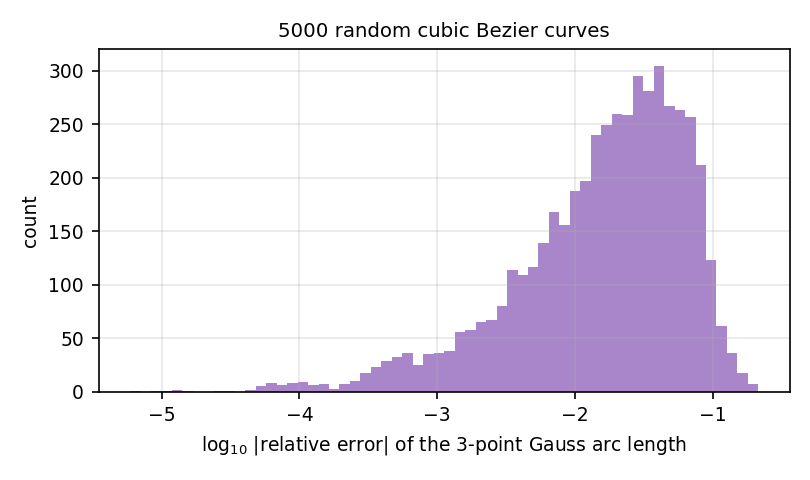
\includegraphics[width=\textwidth]{ch4f-gauss.png}
\scriptsize Use more nodes, or subdivide a curve (de Casteljau at $t = \frac12$ gives the two halves) until the rule converges, or measure the length on a fine polyline, as \code{svg\_to\_vertex.py} does. The notes' own test (section 15) shows the error: 103.164 for the wing's quadratic, whose length is 104.648 ($-1.4$\,\%).
\end{columns}
\sourcecredit{Senter's design notes, section 6; \code{tools/ch4f\_figures.py}.}
\end{frame}

\begin{frame}{From SVG space to the simulation box}
\label{fr:map}
\footnotesize
SVG space $S = [0, w] \times [0, h]$ has its origin top left, $y$ down; the experiment $E = [0, L_x] \times [0, L_y]$ has it bottom left, $y$ up. The notes' affine map (written as a $3 \times 3$ matrix, as the SVG standard writes transforms; the notes print its translation entry as $h$, which is right only when $h = L_y$):
\[ T: (x, y) \mapsto \Big( \frac{L_x}{w}\,x,\ \ L_y - \frac{L_y}{h}\,y \Big). \]
Example: $(10, 60)$ in $[0, 100]^2$ goes to $(0.1, 0.4)$ in $[0, 1]^2$. B\'ezier curves are invariant under affine maps, so control points can be mapped first and the curve meshed in $E$ (or meshed in $S$ with $\Delta s$ mapped back).
\begin{itemize}
  \item MeshmerizeMe reads $L_x$, $L_y$ and $N_x$ from an \code{input2d} in the SVG's folder (IB2d's format; other keys are ignored) and sets $\Delta s = \frac12\,\Delta x = L_x/(2N_x)$; it expects $\Delta x = \Delta y$ but not a square box. The \code{.vertex} file is named from \code{string\_name}, whatever the SVG is called.
  \item The map $T$ stretches each axis separately: when $w/h \ne L_x/L_y$, the shape is distorted. Make the drawing's aspect ratio match the box, or map with one scale (\code{svg\_to\_vertex.py --fit uniform}, its default) and place the object afterwards.
  \item IB2d's SVGs do not start at the origin (the starfish's \code{viewBox} starts at $(102.08, 20.94)$): map $[x_{\min}, x_{\min} + w] \times [y_{\min}, y_{\min} + h]$, not $[x_{\min}, w] \times [y_{\min}, h]$ as the notes' section 12.1 has it (slide \ref{fr:nodes}).
\end{itemize}
\sourcecredit{Senter's design notes, sections 11 and 12.1; Senter et al.\ (2021), section 2.2 and appendix B; the IB2d SVG files.}
\end{frame}

% ---------------------------------------------------------------- MeshmerizeMe
\begin{frame}{MeshmerizeMe: points at equal distances}
\label{fr:mm}
\footnotesize
For each B\'ezier curve $\gamma$, find parameters $0 \le t_1 < \cdots < t_n \le 1$ with equal \al{Euclidean} distances
\[ d(t_i) = \|\gamma(t_{i+1}) - \gamma(t_i)\| = \Delta s, \qquad i = 1, \ldots, n - 1, \]
by gradient descent on the mean squared relative error
\[ J(t) = \frac{1}{2(n-1)} \sum_{i=1}^{n-1} \Big( \frac{d(t_i) - \Delta s}{\Delta s} \Big)^2, \qquad t^{\text{new}} = t^{\text{old}} - \alpha\,\nabla J(t), \]
with a variable learning rate $\alpha$ (the paper gives $\partial J/\partial t_j$ in full). The number of points is estimated as the arc length over $\Delta s$. All paths of the file are merged into one poly-B\'ezier path, split into sub-paths of equal arc length processed in parallel, each seeded with $n = L_{sp}/\Delta s$ points; the command line sets the learning rate, the convergence threshold, and the number of points per sub-path (\code{num-points}).

\al{Errors}: on 5000 SVG files with one random cubic each (a $1000 \times 1000$ pixel drawing onto a $1 \times 1$ box at $256 \times 256$, default settings), the median relative spacing error per curve averaged 3.2\,\%, its middle half 2.6--3.5\,\%. Strongly curved sub-paths may get too many points (use \code{num-points}); separate objects in one file get a large error at the jump between them.
\sourcecredit{Senter et al.\ (2021), section 2.2 and 2.2.1, equations (1)--(4) and figure 3.}
\end{frame}

\begin{frame}[fragile]{Installing and running it}
\label{fr:install}
\begin{columns}[T]
\column{0.5\textwidth}
\footnotesize
From the project's main folder (a clone of \url{https://github.com/dmsenter89/MeshmerizeMe}):
\begin{lstlisting}[style=shell]
pip install .
# or, in a virtual environment with the
# supplied requirements:
pip install . --no-deps
pip install -r requirements.txt
\end{lstlisting}
Both scripts are put on the path (on Linux and Mac). Python 3; the paper names OpenCV, Tkinter (the GUI; part of Python, not a pip package) and Matplotlib; \code{requirements.txt} was not read here. ``This version will only handle 2D code.''
\column{0.48\textwidth}
\footnotesize
With the SVG and an \code{input2d} in one folder:
\begin{lstlisting}[style=shell]
MeshmerizeMe.py simple.svg
# batch: a list of files, or a pipe
find . -name '*svg' | MeshmerizeMe
\end{lstlisting}
``That's it! Just make sure an input2d file is also present in the same folder as the SVG image.'' A minimal \code{input2d} for MeshmerizeMe needs only \code{Nx}, \code{Lx}, \code{Ly} and \code{string\_name} (the paper's four lines, for $[0, 0.5]^2$ at $64 \times 64$); a simulation needs the rest of IB2d's keys. MeshmerizeMe's plotting tool shows the \code{.vertex} file to check the geometry. The wiki's script is \code{MeshmerizeMe.py}, the paper's \code{MeshmerizeMe}; the pipe line is from the notes' wish list (section 2), the batch mode and the pipe are confirmed by the paper.
\end{columns}
\sourcecredit{The 2021 lecture, slides 4, 5 and 7 (with the project's documentation pages ``Installation-Instructions'', ``The-ContourizeMe-Script'', ``The-MeshmerizeMe-Script''); Senter et al.\ (2021), section 2; the batch line from Senter's notes, section 2.}
\end{frame}

% ---------------------------------------------------------------- the IB2d examples
\begin{frame}{What IB2d ships: \code{Example\_Meshmerize\_Me}}
\label{fr:ib2dex}
\scriptsize
\begin{tabular}{@{}L{0.24\textwidth}L{0.68\textwidth}@{}}
\toprule
folder & contents \\
\midrule
\code{Dragonfly\_Wing} & the paper's first example: \code{Images/} (the cropped wing as png and svg, the Chan--Vese contour), \code{Wingitize\_Me.m}, \code{wing\_flow.vertex} (MeshmerizeMe's points), \code{wing\_vein.vertex}/\code{.target} (the simulation's), \code{please\_Compute\_External\_Forcing.m}, \code{input2d}, \code{main2d.m} \\
\code{Insect\_Wing\_Veins} & the same case, copied earlier (2018): the same \code{Wingitize\_Me.m}, \code{.vertex} and \code{.target} files; \code{cropped\_wing.svg} and its optimised version; $\mu = 0.1$, $T = 1$ (Dragonfly: 0.01, 10) \\
\code{Flow\_Around\_Starfish} & the first starfish (May 2019, ``still working out kinks''), ported here: \code{starfish\_initial.svg}, \code{\_cleaned.svg}, \code{\_final.svg}, \code{star\_flow.vertex} (MeshmerizeMe's points), the MATLAB script that places them in a channel (\code{modify\_read\_Vertex\_Points\_and\_Plot\_Them\_and\_Print\_Them.m}), \code{starfish\_flowtank.vertex}/\code{.target}, the forcing, a VisIt session, and \code{MeshingTutorial.md} \\
\code{Starfish} & the paper's third example (its section 3.3; August 2019): the same SVGs and \code{star\_flow.vertex}; the starfish at $x = 0.5$ on targets ($5 \cdot 10^5$) and springs, a 2\,Hz sine ($U_{\max} = 500$, $w = 0.23$), $T = 3$ \\
\code{old}, top level & a leaf: \code{optimal\_leaf.svg}, \code{Leafitize\_Me.m}, \code{leaf\_flow.vertex}, \code{leaf\_vein.vertex}/\code{.target} \\
\bottomrule
\end{tabular}

\footnotesize All MATLAB (Octave cannot run matIB2d, chapter 4a). \code{MeshingTutorial.md} is unfinished: it finds the image, runs ContourizeMe, ``play with the levers until the contour seems to match'', opens the SVG in Illustrator or Inkscape, and stops mid-sentence at the clean-up (a last heading holds only a plot of \code{star\_flow.vertex}).
\end{frame}

\begin{frame}{The starfish example's MATLAB pipeline, read}
\label{fr:pipeline}
\footnotesize
\code{modify\_read\_Vertex\_Points\_and\_Plot\_Them\_and\_Print\_Them.m} of \code{Flow\_Around\_Starfish} turns MeshmerizeMe's \code{star\_flow.vertex} (3839 points) into the channel case (the \code{Starfish} folder's copy differs in step 3 and the target stiffness, and adds springs: slide \ref{fr:ib2dex}):
\begin{enumerate}
  \item scale the points so that their \emph{mean} spacing becomes $\Delta s = L_x/(2N_x) = 1/2048$ (for $1024 \times 1024$ on $[0, 1]^2$), then by $0.25$ (a smaller starfish);
  \item keep every \code{skip}-th point, \code{skip = ceil(ds\_Desired/ds\_Check)} $= 4$: 960 points, spacing back near $\Delta s$ on average (the ratio is 4 only up to rounding: computed with NumPy's \code{mean} it is $4 + 9 \cdot 10^{-16}$ and \code{ceil} gives 5, 768 points; MATLAB's rounding went the other way, as the 960 shipped points show);
  \item move the centroid (the mean of the points) to $(0.3125, 0.125)$: a starfish $0.080 \times 0.074$ at mid-height of the $1 \times 0.25$ channel, a third of the way along;
  \item add two walls at $y = 0.01$ and $0.24$ with points $2\,\Delta s$ apart (1025 each, from $x = 0$ to 1, two places that are one in the periodic box: each wall has a doubled point), and write targets: $2.5 \cdot 10^5$ on the starfish, $2 \cdot 10^7$ on the walls (MATLAB's 1-based indices).
\end{enumerate}
\begin{punchbox}
\small Three things to know: the starfish's spacing is whatever MeshmerizeMe's was, thinned (next slide); the walls' points are $2\Delta s = \Delta x$ apart, one per cell of the $1024 \times 256$ grid, not the two per cell of the rule; and the hard-coded $L_x = L_y = 1$, $N_x = 1024$ of step 1 must match the flow tank's $\Delta x$ ($1/1024$ there too) by hand.
\end{punchbox}
\end{frame}

\begin{frame}{How even are the points?}
\label{fr:spacing}
\centering
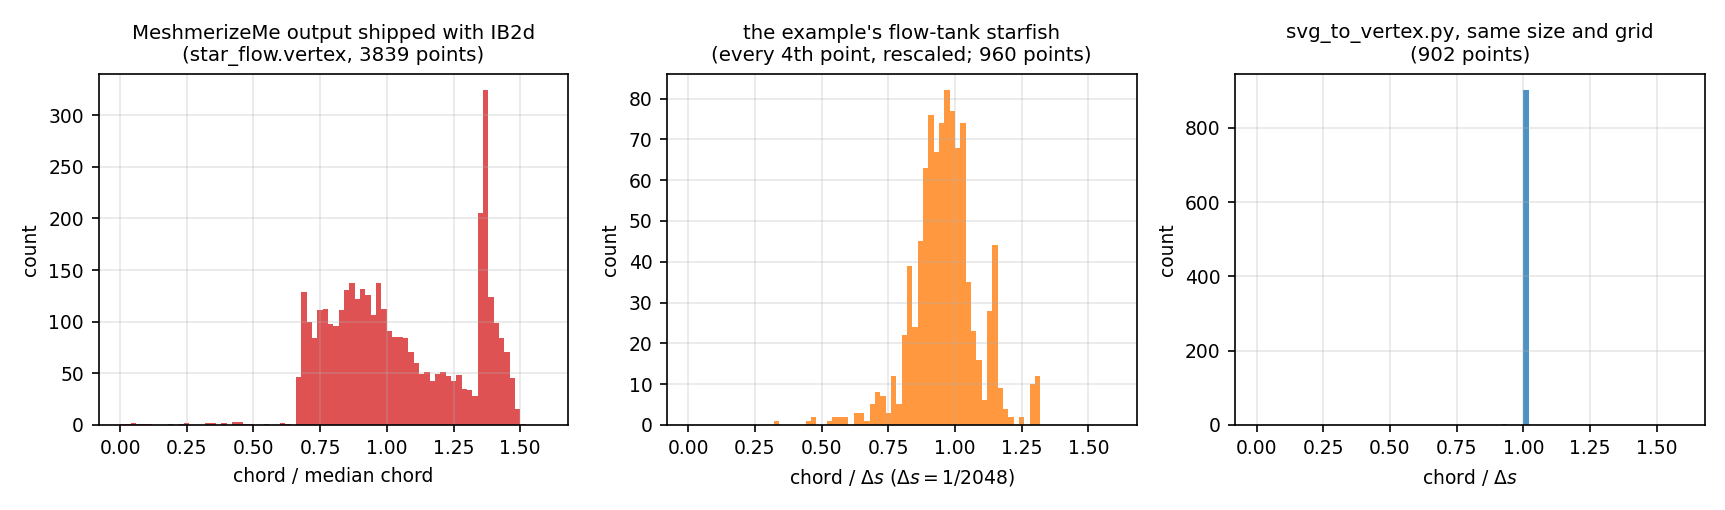
\includegraphics[width=0.90\textwidth]{ch4f-spacing.png}

\footnotesize
\begin{columns}[T]
\column{0.5\textwidth}
\al{MeshmerizeMe's \code{star\_flow.vertex}} (3839 points, one per path piece of the cleaned SVG: its nodes, slide \ref{fr:nodes}): chords from 0.015 to 1.51 times their median, 5th--95th percentile 0.70--1.42. \al{The example's flow-tank starfish} (every fourth point, rescaled): 0.34--1.31 $\Delta s$, 5th--95th 0.77--1.15.
\column{0.48\textwidth}
\al{\code{svg\_to\_vertex.py}} on the same SVG, the same size and grid: 902 points, every chord 1.001 $\Delta s$ but the closing one (0.92). The shipped file's spread does not match the paper's 3.2\,\% typical error; it may predate the version the paper describes (slide \ref{fr:nodes}).
\end{columns}
\sourcecredit{\code{tools/ch4f\_figures.py}.}
\end{frame}

\begin{frame}{What the shipped \code{star\_flow.vertex} is}
\label{fr:nodes}
\footnotesize
\begin{itemize}
  \item Its 3839 points are exactly the first points of the 3839 pieces of \code{starfish\_final.svg}, mapped by
  \[ x' = 0.5\,\frac{x - 102.078}{1217.029 - 102.078}, \qquad y' = 0.5\,\frac{1152.080 - y}{1152.080 - 20.939}. \]
  \item The four numbers are the drawing's \code{viewBox}: $x_{\min}$, $y_{\min}$, width, height. The map reads them as $x_{\min}$, $y_{\min}$, $x_{\max}$, $y_{\max}$, the reading of the notes' section 12.1 (``$[x_{\min}, \text{width}] \times [y_{\min}, \text{height}]$''), into a $0.5 \times 0.5$ box (the box of the plot in \code{starfish\_mesh\_image.png}). It stretches $x$ by 1.45\,\% against $y$, and the MATLAB example inherits the stretch.
  \item At $256 \times 256$ on $[0, 0.5]^2$ (the MATLAB script's note: ``original resolution set at 256x256'') $\Delta s = 0.5/512$, and no piece is longer than 1.02\,$\Delta s$ (median 0.67\,$\Delta s$): a count of points made path by path, arc length over $\Delta s$ as the paper estimates it (section 2.2), is at most about one per piece, and the file has exactly one per piece. The version the paper describes merges the paths first (section 2.2.1). The file was committed in May 2019 and the paper received in November 2019: it may predate that version.
  \item The lesson: plot and measure the points you are given (chord$/\Delta s$, previous slide), not only the outline they follow.
\end{itemize}
\sourcecredit{\code{star\_flow.vertex} and \code{starfish\_final.svg} of \code{Flow\_Around\_Starfish}; Senter's notes, section 12.1; Senter et al.\ (2021), section 2.2.}
\end{frame}

\begin{frame}{The two point sets on top of each other}
\label{fr:overlay}
\centering
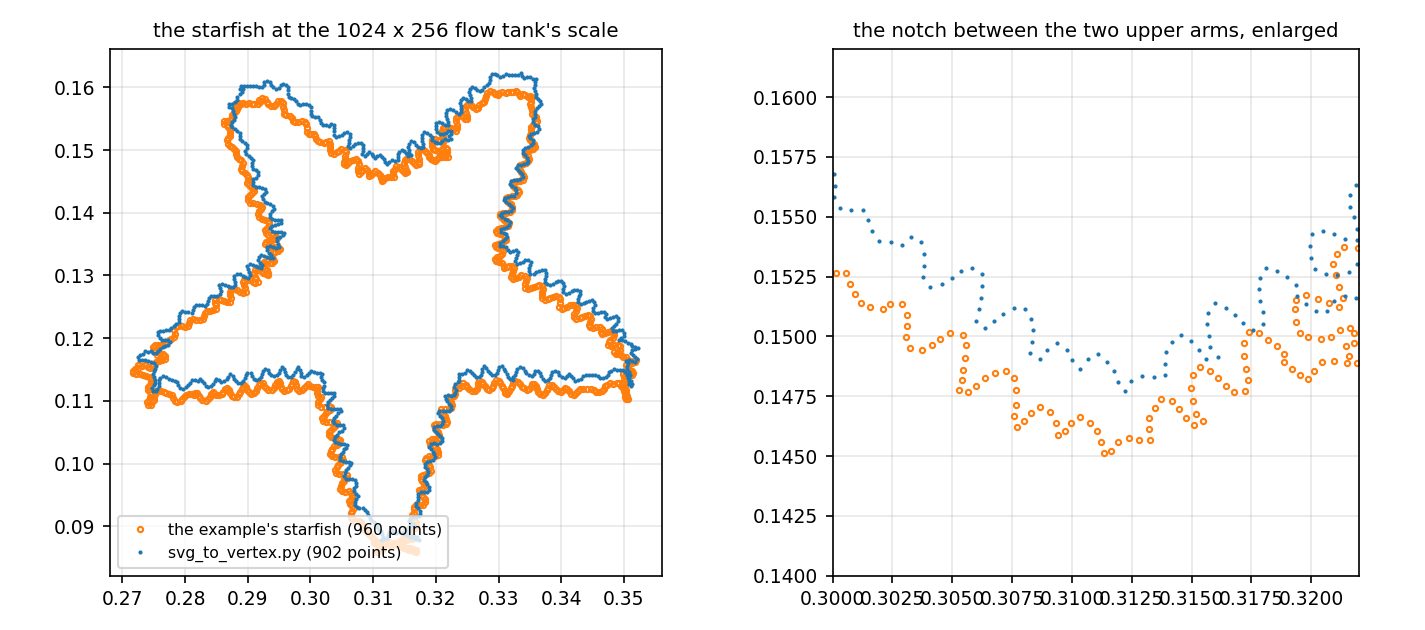
\includegraphics[width=0.74\textwidth]{ch4f-overlay.png}

\small
Same outline and size (orange: the example's 960 points; blue: \code{svg\_to\_vertex.py}'s 902), but the MATLAB script centres the mean of its points and the sampler its bounding box, so the blue set sits 0.0025 higher, and the orange one is 2\,\% wider for its height (slide \ref{fr:nodes}). Enlarged at the notch between the two upper arms (right), the orange points bunch and gap; the blue ones are $\Delta s$ apart along the traced outline. Both follow the SVG; neither is more ``accurate'' than the tracing, which has pixel-scale wiggles of its own.
\sourcecredit{\code{tools/ch4f\_figures.py}.}
\end{frame}

% ---------------------------------------------------------------- the sampler
\begin{frame}[fragile]{A sampler of our own: \code{svg\_to\_vertex.py}}
\label{fr:sampler}
\begin{columns}[T]
\column{0.5\textwidth}
\footnotesize
\begin{enumerate}
  \item Read every \code{<path>} (and lines, polylines, polygons, rectangles without rounded corners, circles, ellipses); parse M L H V C S Q T A Z, absolute and relative, with the traps of slide \ref{fr:svgpath}; arcs become cubics.
  \item Join consecutive pieces whose start is the previous end: ContourizeMe's thousands of pieces become one curve per outline.
  \item Map to $[0, L_x] \times [0, L_y]$, one scale by default (\code{--fit stretch} for the notes' map), then optionally \code{--size} and \code{--center}.
  \item Walk along each finely sampled curve placing the next point at Euclidean distance $h$ from the last (a circle--segment intersection); find $h \approx \Delta s$ by bisection so the last chord, to the end or back to the start, is $h$ too; retry other starting points, and fall back to equal arc length if a hook prevents an even close (it says so).
\end{enumerate}
\column{0.48\textwidth}
\begin{lstlisting}[style=tiny]
python3 svg_to_vertex.py drawing.svg --plot
python3 svg_to_vertex.py \
    starfish_final.svg --input2d input2d \
    --size 0.0803 --center 0.3125,0.125
\end{lstlisting}
\scriptsize
\begin{tabular}{@{}l@{\hspace{5pt}}r@{\hspace{5pt}}l@{}}
\toprule
SVG (unit box, $256^2$) & points & chord$/\Delta s$ \\
\midrule
the notes' wing & 801 & 1.0005 \\
circle, $r = 0.4$ & 1287 & 0.9999 \\
starfish (final) & 2469 & 0.9996 \\
dragonfly wing (Images) & 4253 & 0.965--1.010 \\
insect wing veins & 5038 & 0.992--1.038 \\
leaf (old) & 2321 & 0.32--1.001 (1 fallback) \\
\bottomrule
\end{tabular}

\vspace{0.5mm}
The circle's 1287 points match $2\pi r/\Delta s = 1286.8$. Step 4's last chord is $h$ within the script's 0.8--1.25\,$h$ (the starfish: 0.92 and 1.13\,$\Delta s$, slides \ref{fr:spacing}, \ref{fr:starcase}); step 2 joins ends within $10^{-5}$ of the drawing's size (\code{--merge-tol}). The (optimised) wing veins need it: rounding left their pieces' ends up to 0.001 apart; at $10^{-6}$, the first default, they stayed 240 open pieces (5245 points, chords 0.85--1.16\,$\Delta s$); joined, 34 contours, as in the unoptimised file.
\end{columns}
\sourcecredit{\code{examples/IB2d/Mesh\_From\_SVG/svg\_to\_vertex.py}; NumPy only (Matplotlib for \code{--plot}).}
\end{frame}

% ---------------------------------------------------------------- the run
\begin{frame}{The starfish in a channel, in Python}
\label{fr:starcase}
\footnotesize
\begin{columns}[T]
\column{0.52\textwidth}
\code{examples/IB2d/Mesh\_From\_SVG/Starfish\_Channel}, a port of the MATLAB example \code{Flow\_Around\_Starfish} at half its resolution:
\begin{itemize}
  \item \code{make\_starfish\_channel.py path/to/starfish\_final.svg}: the outline sampled at $\Delta s = 1/1024$ for $512 \times 128$ on $[0, 1] \times [0, 0.25]$, sized to $0.0803$ and centred at $(0.3125, 0.125)$ as in MATLAB, but by its bounding box (MATLAB: the mean of its points, 0.0025 lower): 405 points; walls at $y = 0.01$ and $0.24$, $\Delta s$ apart (2 $\times$ 1024 points); targets $2.5 \cdot 10^5$ and $2 \cdot 10^7$;
  \item \code{please\_Compute\_External\_Forcing.py}: the MATLAB forcing with the same numbers: in $0.04 \le x \le 0.06$, $0.02 \le y \le 0.22$, a penalty $k = 10^4$ towards $u_x = -U_{\max}\sin(2\pi\cdot 5\,t)\,(\tfrac{L_y}{2} + \tfrac{w}{2} - y)(\tfrac{L_y}{2} - \tfrac{w}{2} - y)$, $U_{\max} = 2500$, $w = 0.25$, during a 0.2\,s pulse, then 0.2\,s at rest: $39\sin(10\pi t)$ on the centre line;
\end{itemize}
\column{0.46\textwidth}
\small
\code{input2d}: $\rho = 1000$, $\mu = 0.1$, $\Delta t = 5 \cdot 10^{-5}$, $T = 0.4$ (one pulse and one rest; MATLAB's runs to 1).

\vspace{2mm}
8000 steps, 223\,s (under four minutes) on the laptop.

\vspace{2mm}
The SVG is not copied into this repository: it is part of IB2d (GPL-3.0) and was extracted by ContourizeMe from a NOAA photograph; the script reads it from your IB2d clone. \code{main2d.py} (IB2d's own file) and the forcing (a port of IB2d's) stay under IB2d's GPL-3.0.

\vspace{2mm}
\code{main2d.py} is the Turek--Hron example's (any pyIB2d run script with external forcing works); the files carry 0-based indices.
\end{columns}
\end{frame}

\begin{frame}{The run: vorticity, and what the penalty achieves}
\label{fr:starrun}
\centering
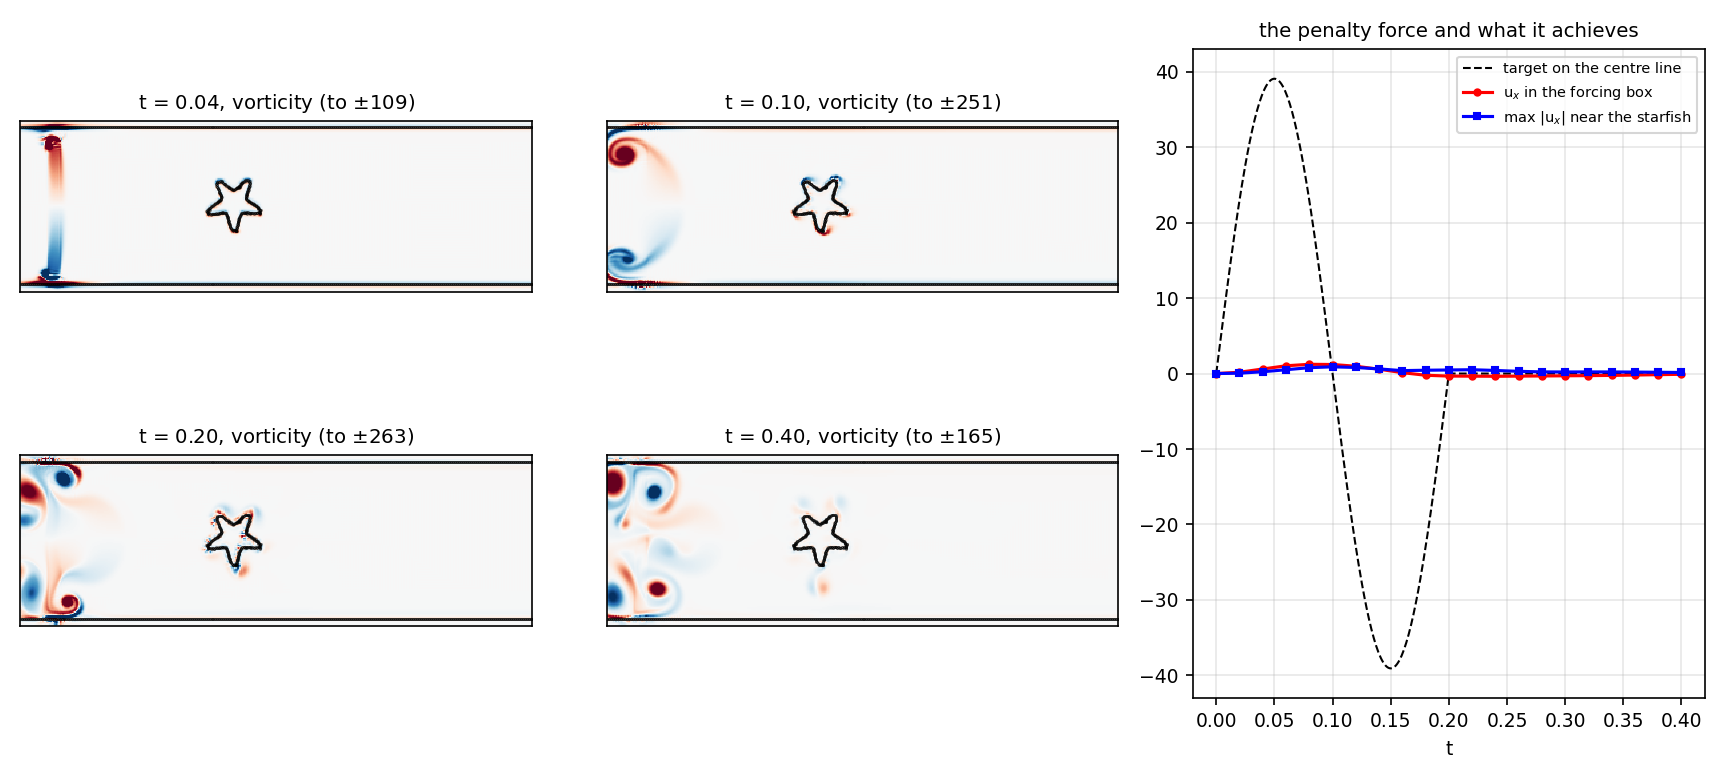
\includegraphics[width=0.68\textwidth]{ch4f-starfish-run.png}

\scriptsize
\begin{columns}[T]
\column{0.5\textwidth}
Left: vorticity at $t = 0.04$, $0.10$, $0.20$ and $0.40$ (each frame on its own scale): the forcing box drives a jet that rolls up into vortex pairs at the walls' ends of the box, a wake forms behind the starfish during the pulse, and the vortices drift back during the rest. Right: the centre-line target (dashed), the speed reached in the forcing box (red) and the largest $|u_x|$ near the starfish (blue).
\column{0.48\textwidth}
The target peaks at 39 at $t = 0.05$; the box reaches 1.23 at $t = 0.08$, \al{3\,\% of the target and some 0.04\,s late}; during the rest the box's centre line flows backwards at about $-0.35$ while the channel is still. Near the starfish $|u_x|$ peaks at 0.89 at $t = 0.10$: with the paper's $L = 0.08$, $Re = \rho L U/\mu \approx 710$ for that local speed, 250 for the flow arriving (slide \ref{fr:penalty}); the paper's 800 (whose $V = 1$\,m/s is ``half the maximum oscillatory inflow speed'') is for its 2\,Hz run. 8000 steps, 223\,s.
\end{columns}
\end{frame}

\begin{frame}{Why the fluid reaches 1, not 39}
\label{fr:penalty}
\footnotesize
\begin{itemize}
  \item \al{The time scale.} The forcing adds $-k(u - u_T)$ to $\rho\,Du/Dt = -\nabla p + \mu\Delta u + f$: on its own it relaxes a parcel of fluid in $\rho/k = 0.1$\,s, half the pulse. A parcel pulled so towards $39\sin 10\pi t$ would reach 16.5 at $t = 0.086$, not 1.23.
  \item \al{The channel.} The fluid in the box cannot speed up alone: between the walls the flux is the same at every $x$ (0.0685--0.0715 at $t = 0.10$), so the box ($10 \times 102$ cells, $0.02 \times 0.2$) has to drive the whole channel ($1 \times 0.23$). Its momentum, $\rho A_{\text{channel}}\,d\bar u/dt \approx k A_{\text{box}} (\bar u_T - \bar u_{\text{box}})$, has the time scale $\rho A_{\text{channel}}/(k A_{\text{box}}) \approx 6$\,s and gives a mean speed of 0.32 at $t = 0.1$; the run has 0.31. The pressure spreads the box's force over all that fluid.
  \item \al{The box.} Its centre line reaches 1.23 with the fluid beside it, next to the walls, flowing back ($-1.6$ to $-2.3$ at $t = 0.08$, $x = 0.05$); downstream the flow is a plug at about 0.3. During the rest the box's centre line stays near $-0.35$ while the channel is still (mean speed $-0.01$): a recirculation.
  \item \al{$U_{\max}$.} The paper's (A.8) divides the parabola by $w^2/4$, which makes $U_{\max}$ the centre-line target; the code does not, so 2500 means 39. The paper's own folder, \code{Starfish}, uses $U_{\max} = 500$, $w = 0.23$: 6.6 on the centre line, at 2\,Hz. How either value was chosen is not recorded.
  \item \al{The Reynolds number}, with the paper's $L = 0.08$: 710 with the largest $|u_x|$ near the starfish (0.89), 250 with the flow arriving at it (0.31), 490 with the paper's own $V$, half the largest inflow speed (half of 1.23). The paper's 800 ($V = 1$\,m/s) is for its 2\,Hz run in \code{Starfish}.
\end{itemize}
\sourcecredit{The run's \code{uX} dumps (slide \ref{fr:starrun}); Senter et al.\ (2021), (A.6)--(A.8); the forcing files of \code{Flow\_Around\_Starfish} and \code{Starfish}.}
\end{frame}

\begin{frame}{Four things the starfish example teaches}
\label{fr:lessons}
\footnotesize
\begin{enumerate}
  \item \al{A penalty is not a boundary condition.} $-k(u - u_T)$ with $k = 10^4$ acting on a fluid of density $10^3$ relaxes a parcel of fluid on a time scale $\rho/k = 0.1$\,s, half the pulse, which alone would allow about 16 of the 39; but the small box has to drive the whole channel (slide \ref{fr:penalty}): the target is 39, the fluid reaches about one. How the shipped $U_{\max} = 2500$ was chosen is not recorded (the code, unlike the paper's (A.8), does not divide by $w^2/4$). Change $\rho$, $k$ or the box and the realised speed changes; measure it (slide \ref{fr:starrun}).
  \item \al{The paper and the files differ:} the paper describes oscillatory flow at 2\,Hz, and the folder it names, \code{Starfish}, has it; the example ported here, \code{Flow\_Around\_Starfish}, committed three months earlier ``still working out kinks'', pulses at 5\,Hz with rests, as above. Read the example's files, not only its description.
  \item \al{Dump 0 of the velocity is transposed} in Python IB2d: \code{u.0000.vtk}, \code{uX.0000.vtk} and \code{uY.0000.vtk} have \code{DIMENSIONS} $N_y\ N_x$, later dumps $N_x\ N_y$ (\code{IBM\_Driver.py} line 668 passes \code{U}, \code{V} untransposed where line 848 passes \code{U.T}, \code{V.T}; \code{Omega}, \code{uMag} and \code{P} are fine). That holds with the \code{vtk} package, as here; pyIB2d's plain-text writer gets \code{u.*.vtk} the other way round. The values are zero at $t = 0$, but on a non-square grid VisIt shows dump 0 with the wrong extent and a reader that trusts the header gets the wrong shape.
  \item \al{Plot and measure what you are given.} The shipped \code{star\_flow.vertex} is the drawing's nodes, one per path piece, mapped with the \code{viewBox} misread (slide \ref{fr:nodes}): its spacing came from the drawing, not from $\Delta s$.
\end{enumerate}
\end{frame}

% ---------------------------------------------------------------- protocol, exercises, summary, references
\begin{frame}{A protocol for a geometry of your own}
\label{fr:protocol}
\small
\begin{enumerate}
  \item \al{Image}: high contrast, little noise, the object whole; crop it to what you will simulate (the dragonfly example opened some veins so flow has an entry and an exit).
  \item \al{Contours}: ContourizeMe (or trace by hand in Inkscape); check the number of contours and their lengths, and delete the noise.
  \item \al{One object, one path}; simplify and flatten transforms before saving.
  \item \al{Points}: MeshmerizeMe or \code{svg\_to\_vertex.py} with the simulation's $L_x$, $N_x$; check the chord statistics (min, median, max of chord$/\Delta s$) and plot the points over the SVG.
  \item \al{Scale and place} with one scale (no stretching), in physical units; size the box so the object is far enough from the periodic edges.
  \item \al{Physics}: targets for rigid parts, springs and beams for elastic ones (chapter 4c's generators), walls at $\Delta s$ too, and the flow (forcing box, its realised speed measured).
  \item \al{Resolution}: re-run the points for a finer grid rather than thinning or rescaling a fine set (chapter 4d).
\end{enumerate}
\end{frame}

\begin{frame}{Exercises}
\label{fr:exercises}
\small
\begin{enumerate}
  \item Trace a leaf, a fin or a wing of your own in Inkscape over a photograph; run \code{svg\_to\_vertex.py} at $64^2$, $128^2$ and $256^2$ and plot the points over the outline. How many points does the outline get at each grid?
  \item Run \code{svg\_to\_vertex.py --fit stretch} on the starfish in a $1 \times 0.25$ box and compare its aspect ratio with \code{--fit uniform}'s.
  \item Write the three-point Gauss rule and a subdividing version (split at $t = \frac12$ until two levels agree to $10^{-6}$); compare their errors on 1000 random cubics.
  \item Re-run the starfish channel with $k = 10^5$ and $10^6$ in the forcing (and $\Delta t$ halved if needed); plot the realised centre-line speed against the target. What $U_{\max}$ gives a peak of 1?
  \item Put three starfish in the channel (the paper's figure 10) by copying and translating the point set; compare the wake of the middle one with a single starfish.
  \item Give the starfish springs and beams between neighbours instead of targets (soft arms), keeping one target at its centre; what does the flow do to the arms? (IB2d's \code{Starfish} folder already gives its starfish springs, $10^7$ between neighbours and $10^5$ across, on top of the targets.)
\end{enumerate}
\end{frame}

\begin{frame}{Summary}
\label{fr:summary}
\footnotesize
\begin{itemize}
  \item MeshmerizeMe turns images into IB geometry in two steps: ContourizeMe finds contours (filters, thresholds, OpenCV contours, Chan--Vese, B\'ezier curves to SVG); MeshmerizeMe reads the SVG and \code{input2d} and writes points about $\Delta x/2$ apart. A vector editor in between cleans the SVG, or replaces ContourizeMe altogether.
  \item SVG paths are poly-B\'ezier curves; parse them carefully (compact numbers, smooth curves, arcs, the flipped $y$), measure lengths on fine polylines rather than with a three-point rule, and map with one scale.
  \item MeshmerizeMe solves for equal Euclidean distances by gradient descent (3\,\% typical error in the paper); the starfish output shipped with IB2d is far less even (its points are the SVG's nodes, slide \ref{fr:nodes}), and the example thins it further. A walk with bisection gives equal chords $h$ within $1/(2n)$ of $\Delta s$ (1.001\,$\Delta s$ for the 902-point starfish), the closing one within the script's 0.8--1.25\,$h$.
  \item From points to a simulation: targets, walls at $\Delta s$, a forcing whose realised speed you measure. The Python port of the starfish ran in 223\,s (under four minutes); the penalty reached about 3\,\% of its target speed in the box, the channel's mean speed less than 1\,\% (slide \ref{fr:penalty}).
  \item Part II ends here. In reading order Part III (IBAMR, chapter 5) comes next; the VisIt part continues with chapter 27.
\end{itemize}
\end{frame}

\begin{frame}{References and credits}
\label{fr:refs}
\scriptsize
\begin{itemize}
  \item D.\,M. Senter, D.\,R. Douglas, W.\,C. Strickland, S.\,G. Thomas, A.\,M. Talkington, L.\,A. Miller, N.\,A. Battista, ``A semi-automated finite difference mesh creation method for use with immersed boundary software IB2d and IBAMR'', Bioinspir.\ Biomim.\ 16 (2021) 016008, \url{https://doi.org/10.1088/1748-3190/ababb0}. Its figures are not reproduced here; figure 1's workflow is redrawn.
  \item M. Senter, ``Creating a Curvilinear Mesh from B\'ezier Curves'', design notes for an early C++ version of MeshmerizeMe (UNC Chapel Hill, about 2017).
  \item MeshmerizeMe: \url{https://github.com/dmsenter89/MeshmerizeMe} and its documentation pages (installation, ContourizeMe, MeshmerizeMe), as presented in the 2021 slides ``MeshMerizeMe''.
  \item IB2d: \url{https://github.com/nickabattista/IB2d}, \code{matIB2d/Examples/Example\_Meshmerize\_Me} (clone at commit 58663e1 of 2024-03-06), and \code{pyIB2d} for the run. The starfish outline was extracted by ContourizeMe from a photograph by J.\,P. McVey (\code{Reef0297.jpg}) of the NOAA Sea Grant Program's Coral Kingdom Collection (Wikimedia Commons), as the paper credits (its reference 47; \code{MeshingTutorial.md} links the same file).
  \item This chapter's code (October 2026): \code{examples/IB2d/Mesh\_From\_SVG} (\code{svg\_to\_vertex.py}, \code{Starfish\_Channel/}, README), \code{tools/ch4f\_figures.py}, \code{wsl/final/ch4f\_star.sh}.
  \item The SVG 1.1 specification (paths, the elliptical-arc implementation notes): \url{https://www.w3.org/TR/SVG11/}.
\end{itemize}
\end{frame}

\end{document}
